\documentclass[10pt]{report}
\usepackage[utf8]{inputenc}
\usepackage[top=2cm, bottom=2cm, left=2cm, right=2cm]{geometry}
\usepackage[francais]{babel}
\usepackage{helvet}
\usepackage[T1]{fontenc}
\usepackage{graphicx}
\usepackage{subcaption}
\usepackage{lmodern}
\usepackage{listings}
\usepackage{amsmath} 
\usepackage{algorithm}
\usepackage[noend]{algpseudocode}
\usepackage{wrapfig}
\usepackage[colorlinks=true, linkcolor=black, urlcolor=blue, breaklinks, pagebackref, citebordercolor={0 0 0}, filebordercolor={0 0 0}, linkbordercolor={0 0 0}, pagebordercolor={0 0 0}, runbordercolor={0 0 0}, urlbordercolor={0 0 0}, pdfborder={0 0 0}]{hyperref}  %désactive les cadres autour des liens
\usepackage{etoolbox}
\usepackage{setspace}
\onehalfspacing
\renewcommand{\familydefault}{\sfdefault}

% Supprime l'espace avant l'en-tête des chapitres
\makeatletter
% les chapitres normaux
\patchcmd{\@makechapterhead}{\vspace*{50\p@}}{}{}{}	
% les chapitres étoilés
\patchcmd{\@makeschapterhead}{\vspace*{50\p@}}{}{}{}
\makeatother



\begin{document}

\begin{titlepage}	
	\flushleft
	\begin{figure}[!h]
		
\includegraphics[height=1.8cm]{Reports/figures/logo_insa_cvl.png}
		\hfill
		
\includegraphics[height=3cm]{Reports/figures/logo_biomedia.png}
	\end{figure}
	\centering
	\vspace{2cm}
	{\scshape\Large Stage industriel de 4ème année\par}
	\vspace{1.5cm}
	{\huge\bfseries Développement d'une bibliothèque mathématique performante pour le traitement d'images médicales\par}
	\vspace{2cm}
	{\Large\itshape Élève ingénieur: François PIAT\par}
		\vspace{1cm}
	\begin{figure}[!h]
		\begin{center}
			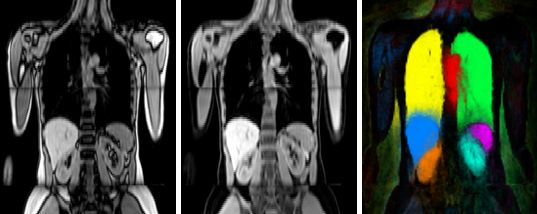
\includegraphics[width=13cm]{Reports/figures/biomedia_image.png}
		\end{center}
	\end{figure}
	\vfill
	\flushleft
	Tuteur INSA: \hfill Tuteurs BioMedIA: \par
	Dr. Julien \textsc{Olivier} \hfill Dr. Ghislain-Anthony \textsc{Vaillant} \\ \hfill Dr. Jonathan \textsc{Passerat-Palmbach}
	\vfill
	% Bottom of the page
	\centering
	{\large Année universitaire 2015 - 2016 \par}
\end{titlepage}

\section*{Remerciements}\newpage
\paragraph*{Résumé} % dans cet ordre
\paragraph*{Mots-clés}
\paragraph*{Abstract}
\paragraph*{Key-words}

\renewcommand\contentsname{Sommaire}
\tableofcontents

\newpage

\chapter*{Introduction}
\addcontentsline{toc}{chapter}{Introduction}

\chapter{Environnement de travail} 
	Cette section détaille l'environnement dans lequel s'est déroulé le stage. Le laboratoire sera d'abord présenté puis le cadre du stage sera introduit.
	\section{Le laboratoire}
	
	\subsection{Imperial College London} 
	L’Imperial College London (officiellement The Imperial College of Science, Technology and Medicine) est une université britannique fondée en 1907 par la fusion du City and Guilds College, de la Royal School of Mines et du Royal College of Science (tous fondés entre 1845 et 1878).\\ ~\par
    L'université possède 9 campus au total, tous situés à Londres, et dont la plupart sont implantés dans des sites hospitaliers.  
    Elle possède 5 départements administratifs et 4 branches techniques: ingénierie, sciences naturelles, business, et médecine.	Le campus principal est localisé dans le quartier du South Kensington, et regroupe la branche d'ingénierie, de sciences naturelles, d'arts et de business. C'est sur ce campus que le département d'informatique se situe. 
    
	\begin{figure}[h!]
		\begin{center}
			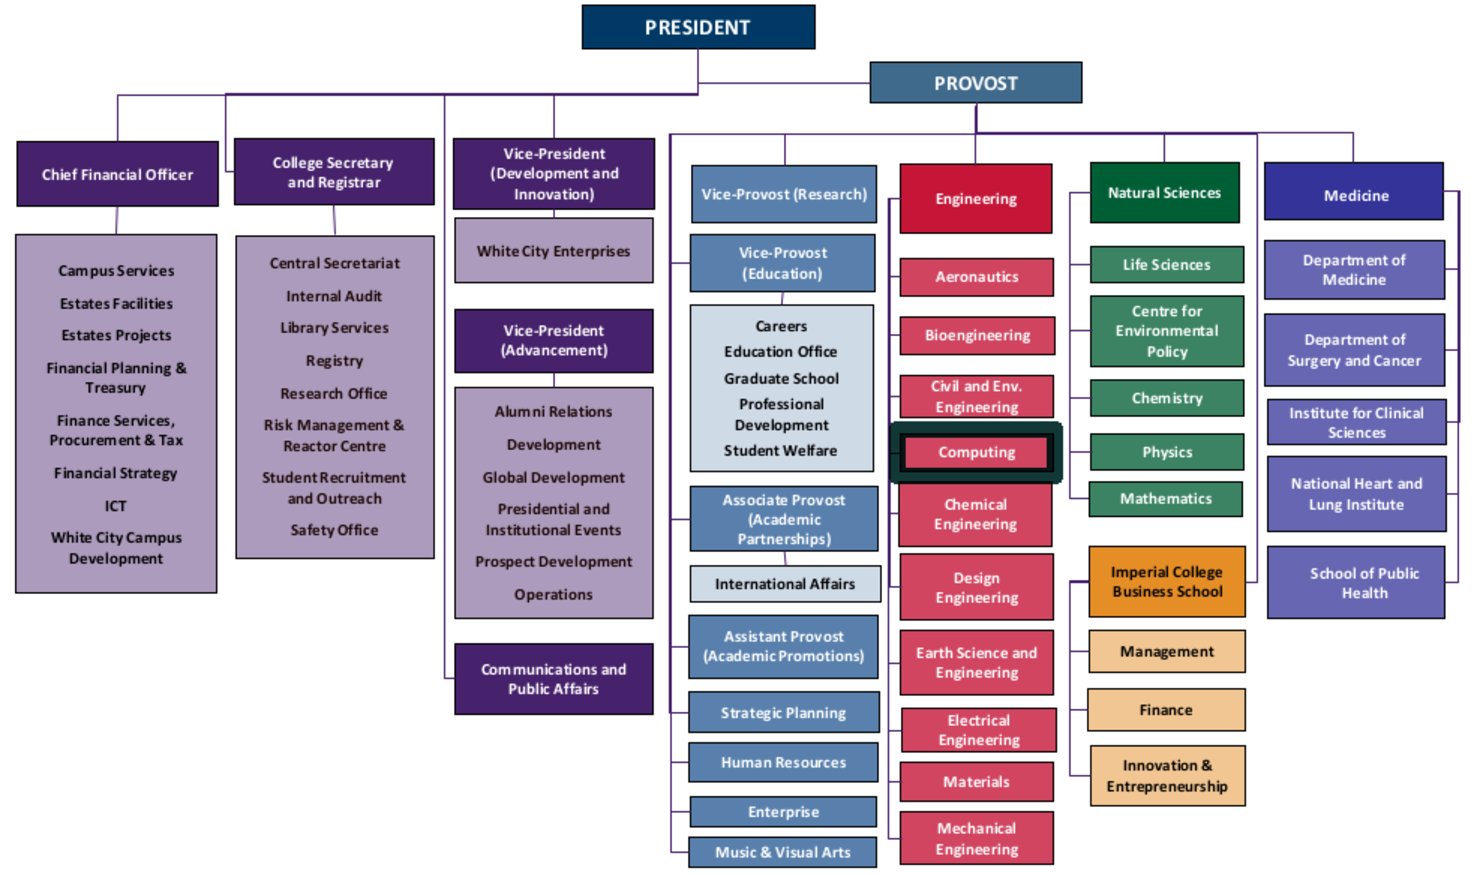
\includegraphics[width=18cm]{Reports/figures/College-Organisation.pdf}
		\end{center}
		\caption[Organigramme de l'Imperial College London]{Organigramme de l'Imperial College London \\ \textit{Le département d'informatique, encadré en noir, se situe dans la branche d'ingénierie (en rouge) de l'université.}}
		\label{Organigramme de l'Imperial College London}
	\end{figure}
	
	\subsection{Le département d'informatique}
	
	Le département d'informatique est divisé en 5 groupes de recherche : 
	\\{$\bullet$}\textit{\textbf{Logic and Artificial Intelligence:}} la recherche en Intelligence Artificielle et Logique englobe des études fondamentales de logique et une variété de disciplines en intelligence artificielle, telles que l'apprentissage automatisé, les flux neurologiques, et la vérification des systèmes autonomes.
	\\{$\bullet$}\textit{\textbf{Distributed Software Engineering:}} la recherche dans le domaine de l'Ingénierie des Logiciels Distribués aborde la conception de systèmes distribués, adaptatifs et fiables.
	\\{$\bullet$}\textit{\textbf{Quantitative Analysis and Decision Science:}} la recherche en Analyse Quantitative et Science de la décision varie de l'optimisation à l'ingénierie de performances, en passant par la des expériences de vérifications quantitatives ou de sécurité.
	\\{$\bullet$}\textit{\textbf{Programming Languages and Systems:}} Systèmes et Langages de Programmation est une section qui combine des travaux théoriques et pratiques en langages et architecture pour obtenir des logiciels rapides, et efficaces.
	\\{$\bullet$}\textit{\textbf{Visual Information Processing:}} la recherche en Traitement d'informations Visualisables couvre une multitude de domaines, incluant la vision numérique, les graphiques, l'apprentissage automatique, et le traitement d'images médicales.
	 
	\begin{wrapfigure}[13]{r}{10cm}
		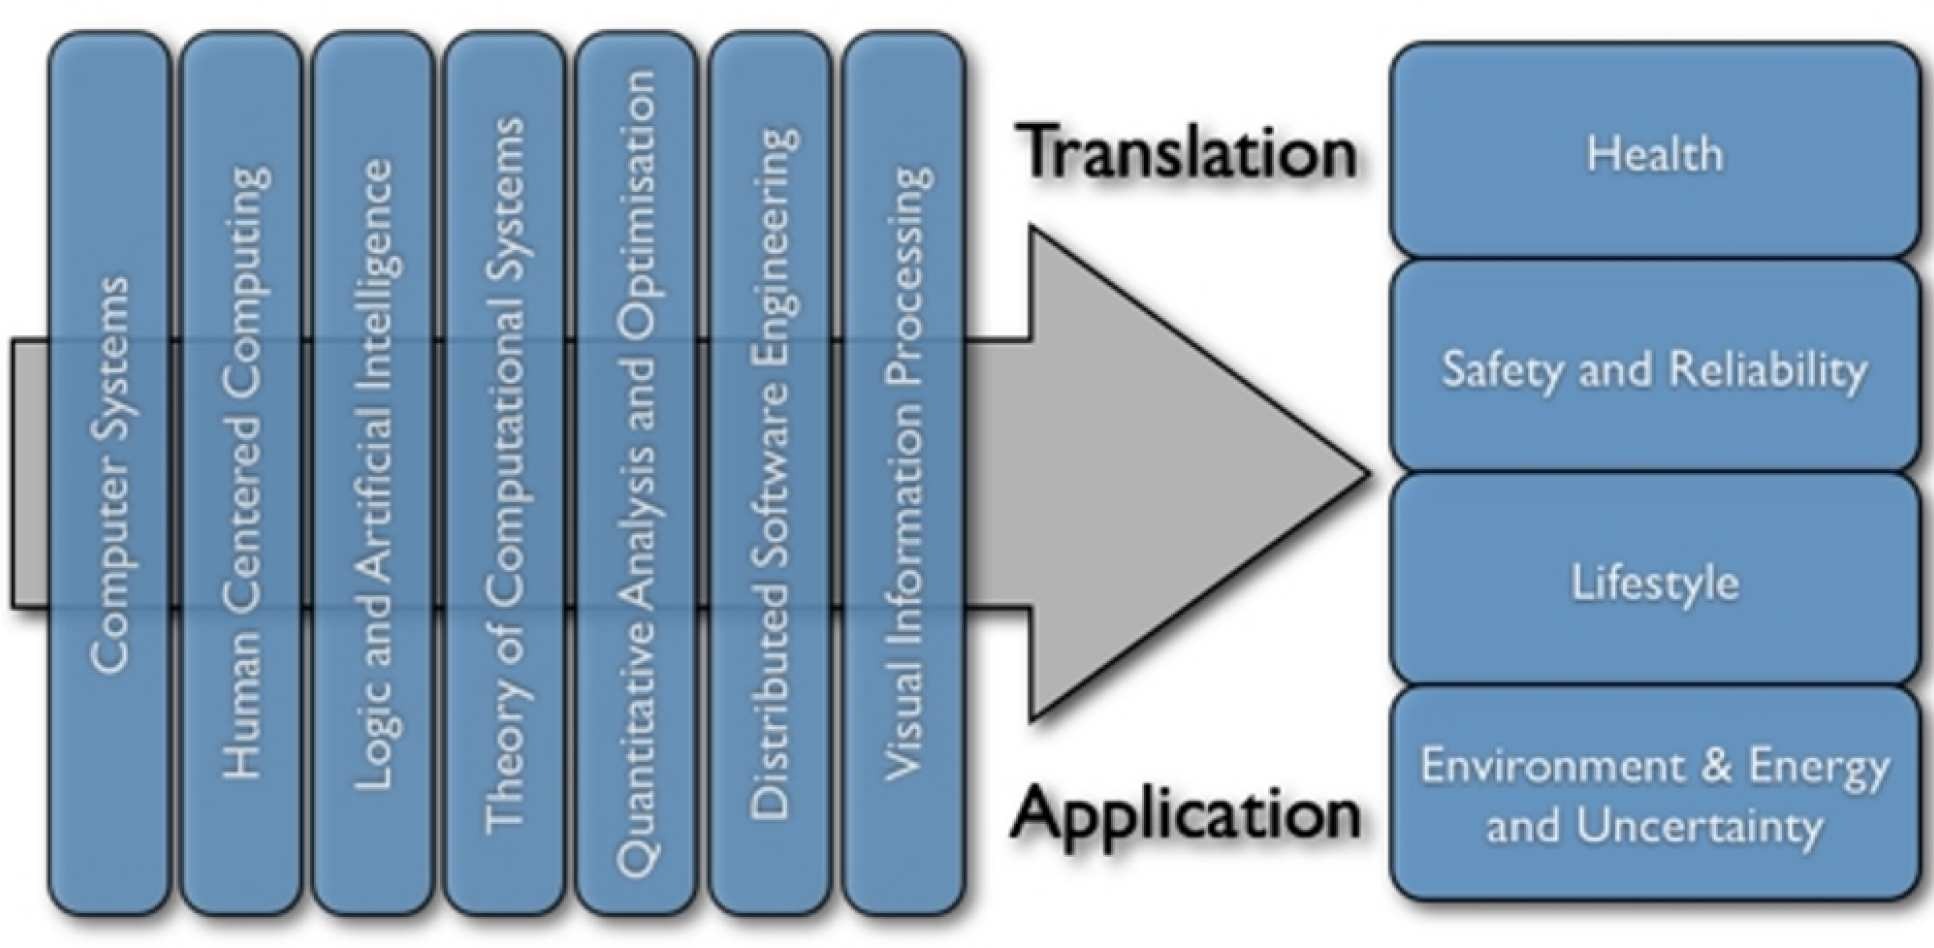
\includegraphics[width=9cm]{Reports/figures/research_strategy.jpg}
		\caption{Stratégie du département de recherche}
		\label{Stratégie du département de recherche}
	\end{wrapfigure}~\par~\par
	
	Les différentes spécialités citées précédemment sont articulées au sein d'un centre de recherche translationnelle, qui se situe à l'intermédiaire entre la recherche fondamentale et la recherche appliquée. La recherche translationnelle s'inspire des travaux de recherche fondamentale et fournit des applications dans les domaines de la santé, de la fiabilité/sécurité, de l'environnement, des modes de vie, de l'énergie et des incertitudes.
	\\
	\\
	\subsection{Le laboratoire BioMedIA}

	La mission du groupe BioMedIA est de développer de nouvelles techniques de
	calcul pour l'analyse d'images biomédicales. Le groupe se concentre sur des
	domaines de recherche de pointe, y compris:\\
	\\{$\bullet$} Le développement d'algorithmes d'acquisition, d'analyse et d'interprétation des images. En particulier dans les domaines du recalage, de la reconstruction,
	du suivi de mouvement, de la segmentation et de la modélisation. \\
	\\{$\bullet$} L'apprentissage machine pour l'extraction d'information clinique à partir
	d'images médicales. Les applications incluent le diagnostic assisté par
	ordinateur, la planification automatisée de traitement médical, ou encore la thérapie et les interventions guidées par ordinateur. \\
	\\Le laboratoire s'intéresse particulièrement à l'imagerie et les technologies de
	traitement informatique qui permet de mieux comprendre le
	développement du cerveau humain, l’évolution des maladies mentales et le
	diagnostic des patients atteints de maladie cardiovasculaire.
	
	\section{Cadre du projet} 
	\subsection{Medical Image Registration Toolkit (MIRTK)}
	Le Medical Image Registration Tool-Kit (abrégé MIRTK) est un logiciel open-source de traitement d'images médicales codé en C++ et utilisé par des chercheurs dans le milieu médical. Le MIRTK prend en charge les formats d'image NIFTI, VTK et PNG. Il propose différents modules qui sont spécialisés pour le recalage d'images. \\ 
	L'utilisation du MIRTK se concentre autour d'une interface en lignes de commandes, incluant le nom de la fonction, les paramètres et les arguments nécessaires, et propres à chacune des fonctions. Par exemple, la ligne de commande suivante permet de rogner une image :
	
	\begin{lstlisting}
mirtk extract-image-region input.nii.gz output.nii.gz -Ry1 200 -Ry2 100
	\end{lstlisting}
	
	\noindent Sur cette ligne de commande:\\
	\t{$\bullet$} \textbf{"mirtk"} indique que la commande à exécuter est une commande du MIRTK.\\
	\t{$\bullet$} \textbf{"extract-image-region"} est la commande désirée. Celle-ci effectue un rognage.\\
	\t{$\bullet$} \textbf{"input.nii.gz"} indique l'emplacement et le nom de l'image d'entrée, idem pour la sortie avec \textbf{"output.nii.gz"}. Ces fichiers sont au format NIFTI (ici compressées).\\
	\t{$\bullet$} \textbf{"-Ry1 200 -Ry2 100"} permet de spécifier la région sur laquelle le rognage est effectué. Ici, dans le cadre d'une étude de la section abdominale par exemple, la hauteur de l'image est réduite à la zone d'étude. \\
	\\L'action de cette ligne de commande est visualisable sur la Figure \ref{Effet de la fonction "extract-image-region"}.
	
	\begin{figure}[h!]
		\centering
		\begin{subfigure}{.5\textwidth}
			\centering
			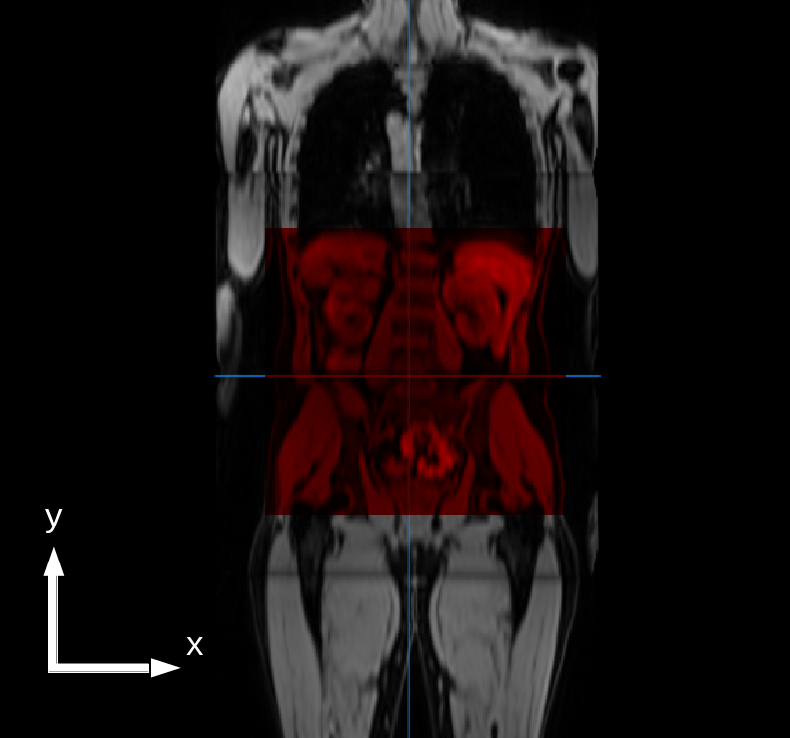
\includegraphics[width=5cm]{Reports/figures/mirtkextractregion1dbis.png}
			\caption{Image d'entrée}
			\label{Image d'entrée}
		\end{subfigure}%
		\begin{subfigure}{.5\textwidth}
			\centering
			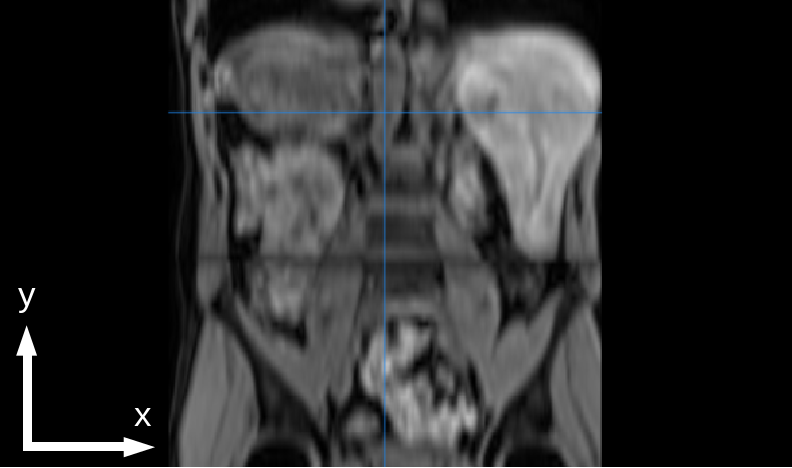
\includegraphics[width=7cm]{Reports/figures/mirtkextractregion21d.png}
			\caption{Image de sortie}
			\label{Image de sortie}
		\end{subfigure}
		\caption{Effet de la fonction "extract-image-region"}.
		\label{Effet de la fonction "extract-image-region"}
	\end{figure}~\par
	
	Le dossier \textit{Applications} du MIRTK regroupe les fichiers correspondants aux commandes exécutables. Ils font appel à certaines dépendances, qui sont réparties en 7 modules : \textit{Common, Image, I/O, Numerics, PointSet, Registration} et \textit{Transformation}. 
	 Le recalage d'image (Registration) est l'une de ses principales fonctions.
	
	 \subsection{UK BioBank}

	 \textit{UK BioBank} est une association fournissant la banque de données médicales la plus importante du Royaume-Uni. Elle a pour but d'améliorer la prévention, le diagnostic et le traitement d'un large éventail de maladies graves, y compris le cancer, les maladies cardiaques, les accidents vasculaires cérébraux, le diabète, l'arthrite, l'ostéoporose, les affections oculaires, la dépression et les formes de démence. 500.000 personnes âgées de 40 à 69 ans ont été recrutées sur la période 2006-2010 à l'échelle nationale pour prendre part à ce projet. Ils ont accepté de donner leur sang, leur urine et des échantillons de salive pour une analyse future, ainsi que des informations détaillées sur eux-mêmes et sur leur santé. D'ici quelques années, ce processus permettra aux chercheurs d'identifier les critères qui influent le développement de certaines maladies.
	 
	 
	 
\chapter{Objectifs et cahier des charges}
	Ce chapitre détaille la motivation du stage, le cahier des charges et la planification des différentes étapes du projet.
	\section{Problématique} 
	Jusqu'ici, le MIRTK a été utilisé pour des études de tailles modestes, dont la validation s'effectue sur une dizaine voire une centaine de patients. Pour cet ordre de grandeur, les performances actuelles du MIRTK sont suffisantes. Cependant avec UK BioBank, cette ordre de grandeur va être multiplié par 10, 100, voire 1000 et le moindre gain de performances, à l'échelle du MIRTK, impactera le temps d'exécution globale sur la base de données UK BioBank.\\ ~\par
	
	Afin d'accélérer leur temps de traitement, les calculs du MIRTK peuvent être effectués sur différents environnement d'exécution:
	\\{$\bullet$}\textbf{ sur une machine en local}, 
	qui distribuera les tâches sur différents cœurs d'exécution et profitera des divers niveaux de cache du processeur pour accélérer les accès mémoire. Les meilleurs processeurs à l'heure actuelle possède quelques dizaines cœurs et jusqu'à 20 MB de mémoire cache.
	\\{$\bullet$}\textbf{une solution d'ordonnancement de tâches informatiques}, tel que SLURM \textit{(Simple Linux Utility for Resource Management)}, qui permettrait de déployer et gérer des tâches simultanément sur plusieurs machines. 
	\\{$\bullet$}\textbf{une grille de calculs}, qui est une infrastructure virtuelle fournissant ensemble de ressources informatiques (dont des environnements d'exécutions) et mise à disposition d'entreprises et/ou de chercheurs. \newline
	Par exemple, les chercheurs du laboratoire BioMedIA utilisent les grilles suivantes : \\
	\t - La grille de l'Imperial College, qui s'étend à tout le réseau de machines de l'université, mais qui est un service payant. Cette grille met au total 5300 cœurs d'exécution à disposition.\\
	\t - La grille européenne, financée par l'Union Européenne et conduite par le CERN, qui met à disposition des services informatiques aux organismes européens de recherche. Ces services comprennent des environnements d'exécutions et plus de 500 PétaBytes de stockage de données (1 Pétabyte = 10\up{15} bytes). Concernant les environnements d'exécution, la grille fournit au total plus de 650 000 cœurs.
	\\{$\bullet$}\textbf{ dans le "cloud"}, c'est-à-dire un service proposé par des entreprises telles que Microsoft ou Amazon, qui permet la location d'un serveur distant, moyennant un certain coût. \\ ~\par
	En revanche, ces différents services possèdent chacun certaines contraintes. L'exécution sur un réseau local, une grille de calculs fournie par l'université ou un cloud implique un coût qui peut rapidement devenir prohibitif. Un slurm ou une grille de calculs mutualisée utilisent les performances d'autres machines, qui, elles-même peuvent éventuellement être déjà occupées par l'exécution d'autres tâches. La réduction du temps d'exécution du MIRTK représenterait un coût moindre dans un cas, sinon un impact plus faible sur les ressources mutualisées.\\ ~\par
	Plusieurs directions sont possibles pour optimiser la durée de ces réquisitions. L'optimisation pourra intervenir au niveau de l'exécution multi-machines: c'est sur cet aspect qu'a travaillé Mr. Maxime Noël, dans le cadre de son stage intitulé:"Interfaçage de fonctions de traitement d'images médicales à une bibliothèque Python et intégration dans un outil de workflow".\\
	\vspace{-0.7cm}

	\begin{figure}[h!]
		\begin{center}
			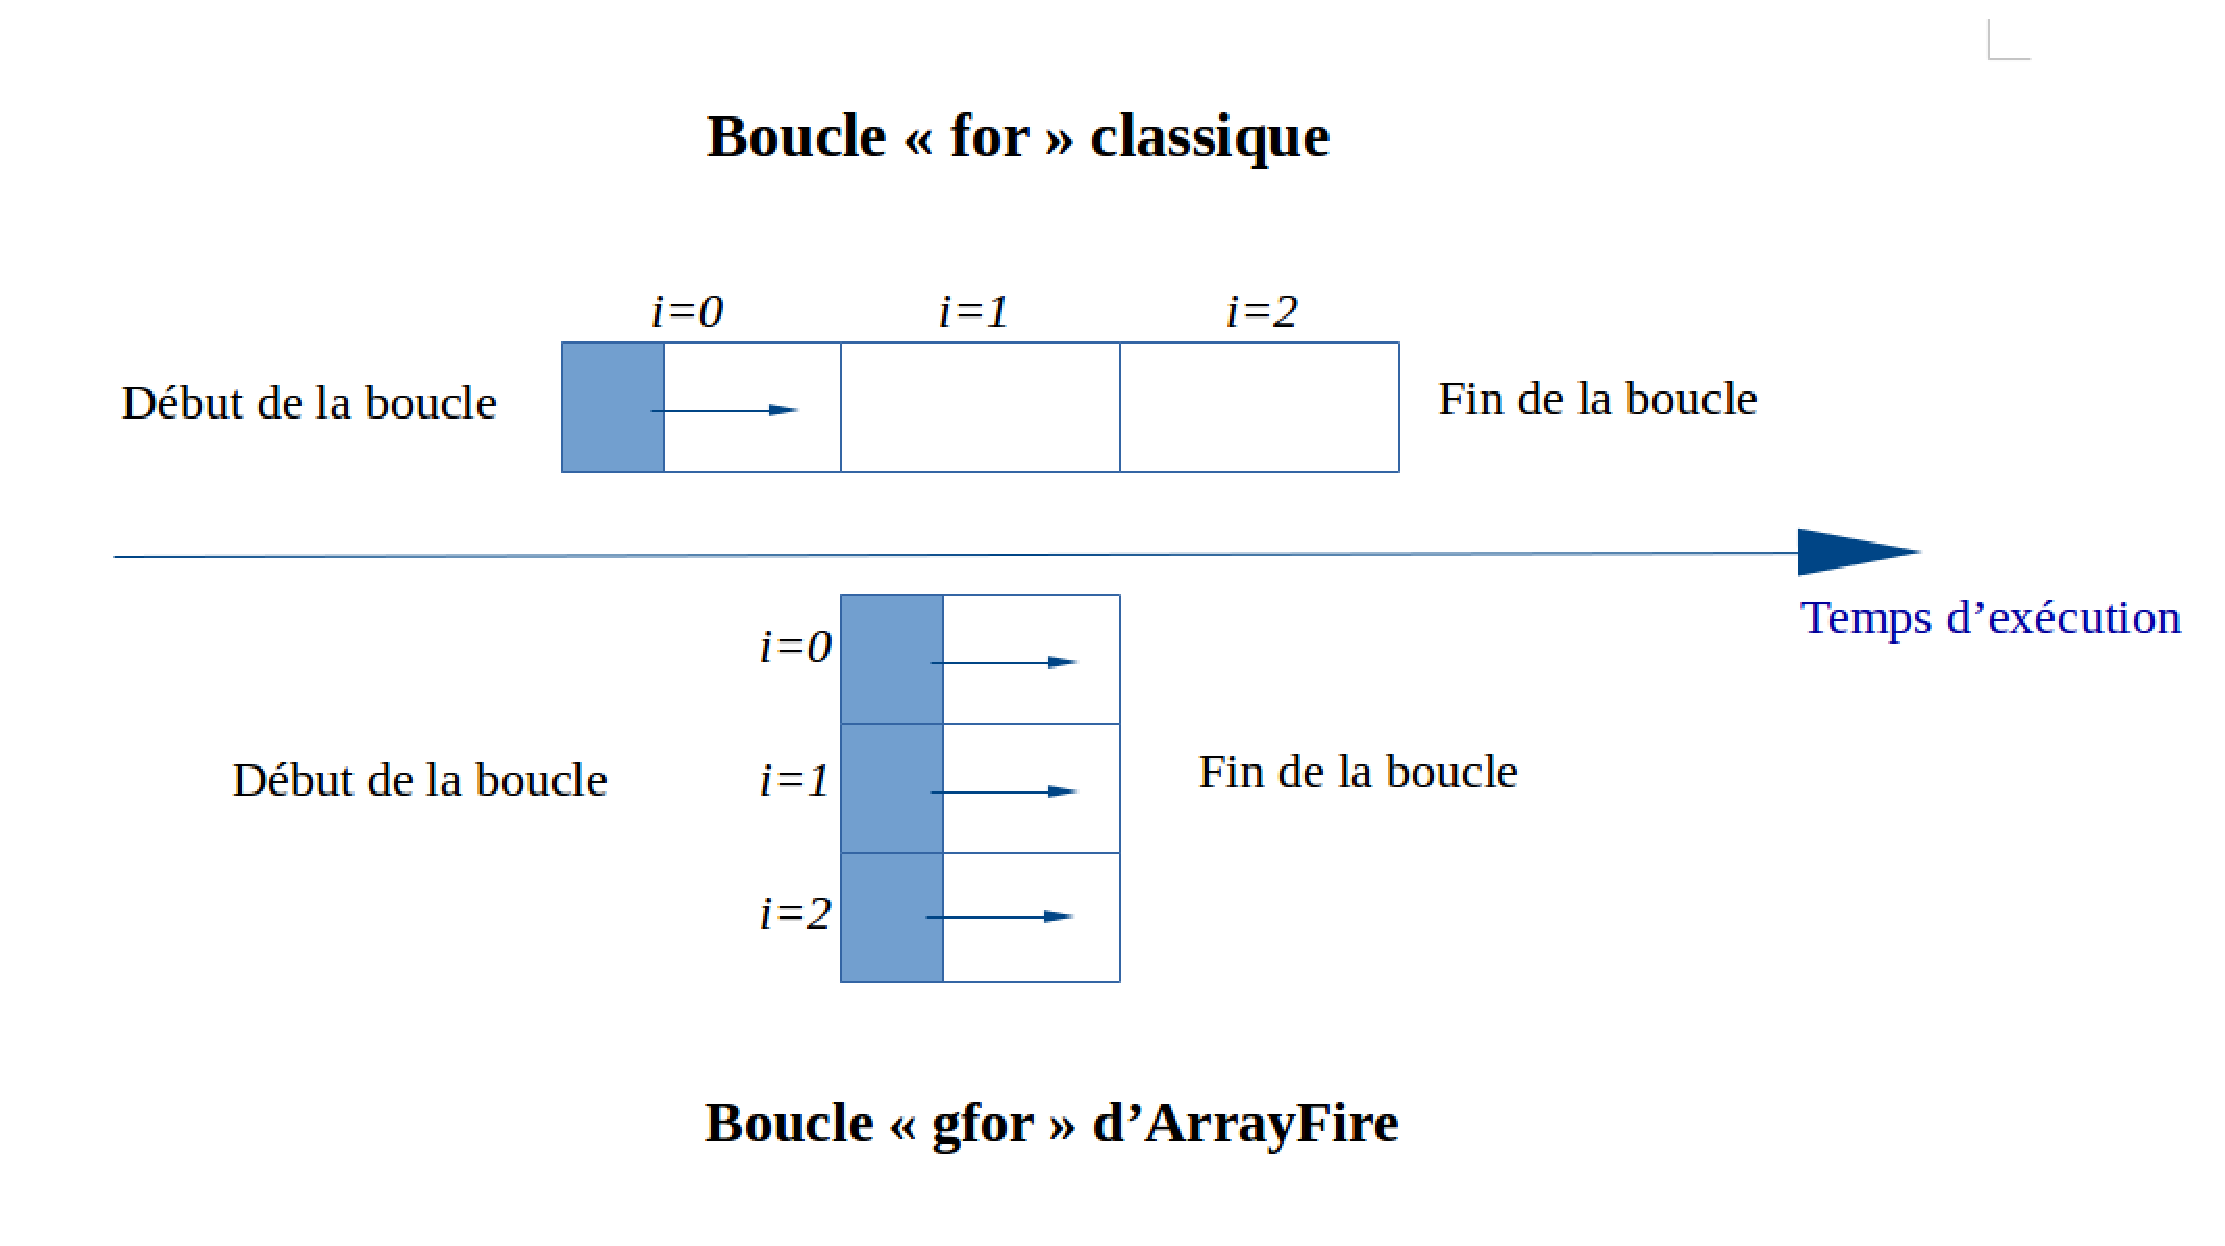
\includegraphics[width=14cm]{Reports/figures/gfor.eps}	
		\end{center}
		\caption{Fonctionnement d'une boucle en parallèle}
		\label{Fonctionnement d'une boucle en parallèle}
	\end{figure}
	~\par~\par
	Une autre possibilité d'optimisation sera la réduction du temps d'exécution sur une machine. Pour cela, le MIRTK utilise une technique d'optimisation appelée "la parallélisation" d'un code. 
	A l'inverse de l'exécution séquentielle, la parallélisation consiste à mettre en œuvre des architectures d'électronique numérique permettant de traiter des informations de manière simultanée, ainsi que les algorithmes spécialisés pour celles-ci. Ces techniques ont pour but de réaliser le plus grand nombre d'opérations en un temps le plus court possible.
	Un algorithme adapté pour la parallélisation partage l'exécution globale d'un programme en plusieurs "blocks" d'exécution, chacun correspondant à un groupe d'instructions. La figure \ref{Fonctionnement d'une boucle en parallèle} ci-contre représente ce principe avec des blocks de 2 itérations.\\

	
	Le calcul par le GPU, ou le GPGPU (General-Purpose computing on Graphics Processing Units) permet de paralléliser les tâches et d'offrir un maximum de performances dans de nombreuses applications : le GPU accélère les portions de code les plus lourdes en ressources de calcul, le reste de l'application étant géré par le CPU. Les applications des utilisateurs s'exécutent ainsi bien plus rapidement.\\
	Pour comprendre les différences fondamentales entre un CPU et un GPU, il suffit de comparer leur manière de traiter chaque opération. Les CPU incluent un nombre restreint de cœurs optimisés pour l'exécution de noyaux complexes, alors que les GPU intègrent des milliers de cœurs conçus pour traiter efficacement de nombreux noyaux simples simultanément.\\
	Les GPU incluent des milliers de cœurs pour traiter efficacement des tâches parallèles. \\ 
	 
	A l'heure actuelle, le MIRTK bénéficie seulement du multi-threading pour l'instant, et nécessite une amélioration sur le plan de ses performances sur plusieurs cœurs. De plus,  le MIRTK n'est pas encore capable d'utiliser d'accélérations matérielles telles que l'utilisation de GPU.
	
	\section{Cahier des charges}
	La réduction du temps d'exécution est l'axe principal de développement du stage. Pour cela, l'amélioration devra se concentrer sur les fonctions élementaires du MIRTK les plus consommatrices en ressource de calcul. Dans le cadre du stage, l'intervention se fera au niveau de son implémentation concrète sur CPU et GPU, appelée "backend" par la suite.\\ ~\par
	
	\noindent Dans le cadre du stage, les besoins suivants ont été définis : \\
	\\{$\bullet$} Adapter l'exécution du MIRTK sur GPU. A l'heure actuelle, le MIRTK utilisent uniquement les quelques cœurs d'un processeur et ne tire pas encore l'avantage des capacités d'un GPU.\\
	\\{$\bullet$} Conserver une exécution transparente du code, en n'altérant ni les lignes de commandes utilisées, ni le résultat attendu.  \\
	\\{$\bullet$} Dans la mesure du possible, un réusinage du code devra être opéré. Suite à la modification du code du MIRTK, ainsi qu'à l'ajout probable certaines fonctionnalités, il est possible que des doublons subsistent, et que la lisibilité de certaines parties du code peut s'améliorer.	
	\section{Planification}
	\subsection{Objectifs} 
	Les objectifs de stage sont définis de la manière chronologique suivante:
	~\par~\par 
	1) \textbf{Étude du MIRTK et de ses dépendances} \\
	Cette étape préliminaire a pour but de comprendre le fonctionnement global du MIRTK et de se familiariser avec son code source. 
	~\par~\par 
	2)\textbf{Analyse de l'interface d'ArrayFire} \\
	Dans le même temps, une analyse de l'interface d'ArrayFire, une bibliothèque mathématique optimisée, et des différentes fonctions proposées par la bibliothèque sera entreprise. Cette étude corrélera les besoins du MIRTK et les solutions proposées par ArrayFire.
	~\par~\par 
	\t 3) \textbf{Intégration de ArrayFire dans le MIRTK} \\
	L'étape fondamentale du stage sera la ré-implémentation de différentes fonctions du MIRTK avec l'intégration des outils apportés par ArrayFire.
	~\par~\par 
	\t 4) \textbf{Analyse des performances} \\
	Un profilage du MIRTK sera effectuée avant et après la modification du code source.
\newpage
	\subsection{Diagramme de GANTT}
	\begin{figure}[h!]
		\begin{center}
			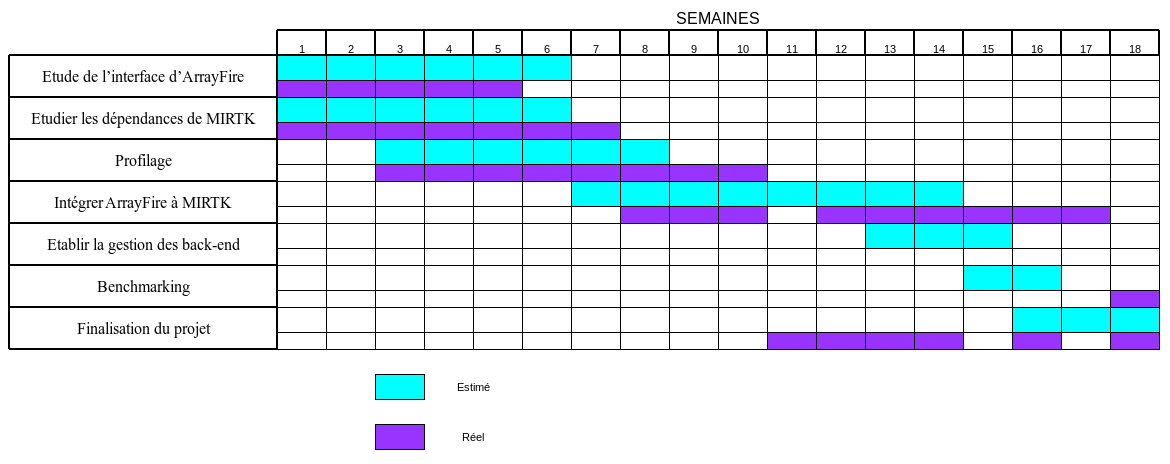
\includegraphics[width=18cm]{ganttchart.png}
		\end{center}	
		\caption{Diagramme de GANTT du stage}
		\label{Diagramme de GANTT du stage}
	\end{figure}
	Durant la première partie du stage, il était convenable de combiner de manière parallèle l'étude de l'interface d'ArrayFire et l'étude du MIRTK. De cette manière, j'ai pu corréler les fonctions utiles dans le MIRTK et les outils semblables disposés par ArrayFire.\\
	Le profilage a ensuite été le lien entre la phase d'étude et celle d'implémentation. \\
	Par manque de temps, la gestion optimisée des backends n'a pas été abordé, afin de finaliser le stage convenablement et d'obtenir tout de même quelques relevés de performances.
\chapter{Réalisation du stage} 

Cette partie du rapport va présenter la bibliothèque ArrayFire, ainsi que son intégration dans le MIRTK.
	\section{Introduction à ArrayFire}
	ArrayFire est une bibliothèque logicielle open-source, proposant une grande variété de fonctions mathématiques optimisées. Elle propose aussi plusieurs fonctionnalités de manipulations de backends afin d'exécuter le même code sur différentes configurations matérielles.
	\subsection{Les fonctions mathématiques}
	L'interface d'ArrayFire repose sur la manipulation d'un type générique de tableau nommé \textit{af::array}. Celui-ci peut contenir tout type de valeurs numériques (entier, flottant ou complexe) et peut être utiliser pour représenter des structures de données allant jusqu'à 4 dimensions, comme des vecteurs, matrices, images, volumes, ou série de volumes. Ce type présente plusieurs constructeurs, et ceux-ci peuvent faire appel à une variable appelée \textit{af::dim4} qui est un ensemble de 4 entiers définissant la taille du \textit{af::array} sur chacune de ses dimensions.\\ ~\par 
	
	\noindent Autour de ce type s'articulent deux types de fonctions:\\ ~\par 
	- Des fonctions mathématiques basiques qui traitent d'algèbre linéaire, telles que des factorisations, décompositions ou opérations de matrices. Jointes à un jeu de fonctions de manipulations de matrices, cet ensemble constitue un noyau de fonctionnalités mathématiques complet. Dans le cas où ArrayFire ne couvre pas une fonctionnalité particulière, il est facile de l'étendre grâce à ces quelques fonctionnalités de base. Pour des fonctionnalités plus complexes, ArrayFire met à disposition un outil appelé \textit{"GFOR"}, qui représente l'équivalent d'une boucle \textit{"FOR"} classique vectorisée. \\~\par 
	- Des fonctions appliquées à divers domaines scientifiques, qui met à disposition des chercheurs en traitement d'images, en traitement du signal, ou en statistiques, une interface pourvue d'outils simple à utiliser. La vectorisation de certaines de ces fonctions peut, grâce à un paramètre supplémentaire, être volontairement activée ou désactivée. Dans le cadre du stage, les fonctions de traitement d'images seront insuffisantes car uniquement appliquées sur des images en 2 dimensions, alors que le MIRTK traite aussi des images en 3 et 4 dimensions. Il sera en revanche possible de s'inspirer de leur implémentation.\\
	
	 %contenu a rajouter 
	~\par 

	\subsection{La gestion des backends}
	
	ArrayFire dispose aussi d'un ensemble de modules permettant de manipuler des backends. \\
	Un premier ensemble de fonctionnalités permet de détecter les backends disponibles pour l'exécution du code.\\ Grâce à cette fonction, il sera possible d'adapter l'exécution du code sur GPU de manière transparente.
	De plus, module de switch de backend dynamique:\\
	+ Infos sur matériel.
	
	
	\section{Intégration de ArrayFire dans le MIRTK}
	\subsection{Filtres concernés}
	La fonctionnalité majeure du MIRTK est le recalage d'images médicales.
	
	Le recalage est une technique qui consiste en la « mise en correspondance d'images », ceci afin de pouvoir comparer ou combiner leurs informations respectives. Cette mise en correspondance se fait par la recherche d'une transformation géométrique permettant de passer d'une image à une autre.
	
	~\par
	Le module de recalage du MIRTK utilise notamment des itérations successives de floutages et de transformations. Pour cette raison, deux fonctions ont été traitées: \textit{smooth-image} et \textit{transform-image}.
	\paragraph{Algorithme de "smooth-image"}
~\par

	\begin{algorithm}[H]
		\caption{smooth-image}\label{smooth-image}
		\begin{algorithmic}[1]
			\Procedure{Naive procedure }{Input pointer, Output pointer, SigmaX, SigmaY, SigmaZ}
				\State $\textit{Initialization InputArray, OutputArray, Kernel}$
				\State $\textit{OutputArray} \gets \textit{Input Pointer}$
				\State $\textit{InputArray} \gets \textit{OutputArray}$
				\If {$SigmaX > 0$} 
					\State $\textit{Initialization KernelX}$	
					\State $\textit{KernelX} \gets \textit{InitializeKernel(SigmaX)}$ \Comment  \textit{InitializeKernel} creates a 1D Gaussian kernel
					\State $\textit{Kernel} \gets \textit{KernelX}$
				\EndIf
				\If {$SigmaY > 0$} 
					\State $\textit{Initialization KernelY}$	
					\State $\textit{KernelY} \gets \textit{InitializeKernel(SigmaY)}$
					\State $\textit{Kernel} \gets \textit{Kernel*KernelY}$

				\EndIf
				\If {$SigmaZ > 0$} 
					\State $\textit{Initialization KernelZ}$	
					\State $\textit{KernelZ} \gets \textit{InitializeKernel(SigmaZ)}$
					\State $\textit{Kernel} \gets \textit{Kernel*KernelZ}$
				\EndIf
				\State $\textit{OutputArray} \gets \textit{convolve3(InputArray, Kernel)}$ \Comment  \textit{convolve3} convolves two 3D matrix 
				\State $\textit{Output pointer} \gets \textit{OutputArray}$
			\EndProcedure
			\State $ $
			\Procedure{Optimised procedure }{Input pointer, Output pointer, SigmaX, SigmaY, SigmaZ}
				\State $\textit{Initialization InputArray, OutputArray}$
				\State $\textit{OutputArray} \gets \textit{Input Pointer}$
				\If {$SigmaX > 0$} 
					\State $\textit{Initialization KernelX}$	
					\State $\textit{KernelX} \gets \textit{InitializeKernel(SigmaX)}$ 
					\State $\textit{InputArray} \gets \textit{OutputArray}$
					\State $\textit{OutputArray} \gets \textit{convolve1(InputArray, KernelX)}$ \Comment \textit{convolve1} convolves one 3D matrix  \& one 1D matrix 
				\EndIf
				\If {$SigmaY > 0$} 
					\State $\textit{Initialization KernelY}$	
					\State $\textit{KernelY} \gets \textit{InitializeKernel(SigmaY)}$
					\State $\textit{InputArray} \gets \textit{reorder(OutputArray, 1, 0, 2)}$ \Comment \textit{reorder} switches dimensions into another order
					\State $\textit{OutputArray} \gets \textit{convolve1(InputArray, KernelY)}$
					\State $\textit{OutputArray} \gets \textit{reorder(OutputArray, 1, 0, 2)}$
				\EndIf
				\If {$SigmaZ > 0$} 
					\State $\textit{Initialization KernelZ}$	
					\State $\textit{KernelZ} \gets \textit{InitializeKernel(SigmaZ)}$
					\State $\textit{InputArray} \gets \textit{reorder(OutputArray, 2, 1, 0)}$
					\State $\textit{OutputArray} \gets \textit{convolve1(InputArray, KernelZ)}$
					\State $\textit{OutputArray} \gets \textit{reorder(OutputArray, 2, 1, 0)}$
				\EndIf
				\State $\textit{Output pointer} \gets \textit{OutputArray}$
			\EndProcedure			
		\end{algorithmic}
	\end{algorithm}
	
	
	\paragraph{Algorithme de "transform-image"}
~\par
	A modifier :
	\begin{algorithm}[H]
	\caption{transform-image}\label{transform-image}
		\begin{algorithmic}[1]
			\Procedure{Homogeneous transform - NN interpolation}{Input pointer, Output pointer, TransformationMatrix, TransformedPointsArray}
			\State $\textit{Initialization InputImageArray, InputWorldArray, TransformationArray, OutputArray}$
			\State $\textit{InputImageArray} \gets \textit{Input Pointer}$
			\State $\textit{InputWorldArray} \gets \textit{InputImageArray *(Input pointer->ImageToWorldMatrix)}$ 
			\State \Comment converts the Image (in pixels/voxels) into a spatial representation (in millimeters)
			\State $\textit{TransformationArray} \gets \textit{TransformationMatrix}$
			\State $\textit{TransformedPointsArray} \gets \textit{InputWorldArray *  TransformationArray}$ 
			\State $\textit{OutputArray} \gets \textit{round(TransformedPointsArray)}$ \Comment Applies the NN interpolation 
			\State $\textit{Output pointer} \gets \textit{OutputArray}$
			\EndProcedure
			\State $ $
			\Procedure{Homogeneous transform - Linear interpolation}{Input pointer, Output pointer, TransformationMatrix, TransformedPointsArray}
			\State $\textit{Initialization InputImageArray, InputWorldArray, TransformationArray, OutputArray}$
			\State $\textit{InputImageArray} \gets \textit{Input Pointer}$
			\State $\textit{InputWorldArray} \gets \textit{InputImageArray * (Input pointer->ImageToWorldMatrix)}$
			\State $\textit{TransformationArray} \gets \textit{TransformationMatrix}$
			\State $\textit{TransformedPointsArray} \gets \textit{InputWorldArray * TransformationArray}$
		    \State $ ???? $
			\State $\textit{Output pointer} \gets \textit{OutputArray}$
			\EndProcedure
		\end{algorithmic}
	\end{algorithm}

	\subsection{Dette technique}

	Le MIRTK est un logiciel dont le code source dérive de celui d'un logiciel plus ancien, appelé IRTK (Image Registration ToolKit). Cependant, peu d'améliorations techniques y ont été ajouté lors de sa refonte en MIRTK. C'est-à-dire que le langage employé, le C++, a été conservé, ou encore que les classes et structures de données ont été simplement étoffées de nouveaux attributs et méthodes. \\
	
	Devenant un logiciel de plus en plus abouti, le code source du MIRTK à renforcé son interdépendance entre ses classes. De son architecture ressort maintenant un couplage "serré", qui, par opposition à un couplage "libre", reflète un agencement de classes très complexe, et qui reste déprécié. Ces interdépendances sont devenues tellement omniprésentes que l'intégration d'ArrayFire dans le MIRTK a dû se restreindre à des fonctions dont l'implémentation est relativement simple. \\
	
	De plus, outre la complexité du code, le MIRTK fonctionne en utilisant des filtres appliqués sur chaque voxel indépendamment. Par exemple, un floutage d'image appliquera un même calcul sur la totalité des voxels de l'image. L'un des problèmes, au niveau des performances de calcul, de cette pratique, est qu'il n'y a que très peu de potentiel d'amélioration. Autrement dit, un logiciel bien optimisé qui utilise cette méthode n'est pas capable d'atteindre les performances d'un logiciel procédant à l'aide de calculs vectorisés. Plus les données à traiter seront importantes, plus le calcul vectoriel devient ainsi rentable.
	
%c++ => langage qui vieillit, programmé en application de kernels successivement sur tous les voxels	//
%Kernels en voxel/voxel => bien qu'optimisé, n'atteindra jamais les performances de fonctions vectorisees.
	

	%	Le contenus des sous-parties, ainsi que d'éventuelles d'autres sous-parties dépendront du résultat du profilage.
	
	\section{Évaluation des performances}
		\subsection{Profilage}
	%	Définir le profilage et expliquer la nécessité d'une telle étape dans ce contexte\newline
Un profilage est une étude de comportement d'un programme lors de son exécution. Cette étape est un relevé de performances du MIRTK, et, de même que toutes les démarches utilisées dans la partie "Evaluation de performances", ne modifie aucunement le code source du MIRTK. 

		\subsubsection{a) Configuration}
			\paragraph{Choix du profileur}~\par

Avant d'effectuer un profilage, il a en premier lieu été nécessaire de choisir le bon outil de profilage. Pour le choisir, ont été définis deux principaux critères:\\
{$\bullet$} Le genre d'informations relevées : dans le cadre du MIRTK il était suffisant de se restreindre au temps d'exécution. En revanche, il était nécessaire d'avoir une fonctionnalité analysant (ou permettant au moins de visualiser) l'exécution parallèle du code. \\
{$\bullet$} L'accès gratuit au programme de profilage, puisqu'il ne sera pas utilisé à long terme.\\
Après recherche en ligne d'outils respectant ces critères, 3 différents logiciels de profilage ont été retenus: le "JIT (just-in-time) profiling tool" issu de l'application VTune, CodeXL et le module "Callgrind" de la suite d'outils Valgrind.\\~\par
\noindent VTune, développé par l'entreprise Intel, possède un ensemble de fonctionnalités d'analyses de performances couplées à des outils d'assistance pour rendre un programme plus performant. \\
CodeXL est un outil qui rassemble deux fonctionnalités principales qui sont le débuggage et le profilage. Il s'agit d'un produit fournit par l'entreprise AMD pour accompagner les développeurs à la fois sur CPU, GPU et APU. Un APU est une unité spécialisée dans l'accélération matérielle.
\\Les fonctionnalités fournies par Valgrind sont similaires à celles de CodeXL. Cependant, Valgrind est un logiciel open-source dont la structure est constituée de différents modules, chacun étant spécialisé pour une fonction précise.\\

Bien que les trois programmes précédents semblaient convenir pour l'étude, un critère pourtant essentiel n'avait pas été pris en compte. En effet il était nécessaire que le profileur soit compatible avec différentes configurations matérielles afin de pouvoir réaliser le profilage d'un même code sur différents machines si nécessaire. VTune étant développé par Intel, il n'est compatible qu'avec des configurations matérielles issue de l'entreprise Intel. Semblablement, CodeXL n'est pas fonctionnel pour des supports physiques non produits par AMD.\\

Finalement, c'est Valgrind qui a été choisi, puisqu'il respecte tous les critères cités précédemment.
 \\
 
 		\paragraph{Caractéristiques techniques du support physique}~\par
 	
 		
% a refaire!!!
%		Lors du début de mon stage, il a fallu que je me familiarise avec les dépendances de MIRTK, mais aussi a son fonctionnement interne. C'est lors de cette étude préliminaire que mon tuteur et moi avons étudié, en plus de la bibliothèque EIGEN (destinée aux fonctionnalité mathématiques), la bibliothèque TBB, qui a pour but de mettre en place une parallélisation d'un logiciel. Constatant qu'ArrayFire était constitué de fonctions mathématiques déjà optimisées sur ce plan, il a été convenu de faire un profilage de MIRTK avant d'y intégrer ArrayFire afin de prioriser les points les plus coûteux en ressources de MIRTK. \\
%	%	Les tests ont été effectués sur une machine dont les caractéristiques sont les suivantes : \newline
%	%	{$\bullet$} \textit{Nombre de coeurs:} 8, 2 threads chacun\newline
%	%	{$\bullet$} \textit{Cadence:} 1.6 GHz \newline
%	%	{$\bullet$} \textit{Nombre de caches:} 4 \newline
%	%	{$\bullet$} \textit{Taille des caches:}32k, 32k, 256K, 8192K \newline
%		%ajouter le maximum de détails (RAM, nom du proc ...)\newline
%		Pour une quantité réduite de tests, et afin de cibler les modèles d'utilisation de TBB à remplacer, on a pris l'une des fonctions les plus sollicitées dans MIRTK, il s'agit d'une fonction nommée \textit{transform-image}, et qui dispose de 5 options, définissant un type d'interpolation mathématique : Linéaire (par défaut), méthode voisin le plus proche (NN), gaussienne, sinus cardinal et B-Spline. \\
%		On notera, de plus, que tous ces tests seront exécutés sur la même machine afin de garder des performances exactement semblables à chaque exécution.
%		
%		Afin de discerner au mieux les performances de MIRTK, le choix du profileur (l'outil faisant le profilage) était important. Le principal poste utilisée pour le profilage travaille sur un processeur INTEL, ce qui nous a convaincu de ne pas utiliser le profileur CodeXl puisque nous avons compris après installation qu'il ne fonctionnait qu'avec des processeurs AMD. On a ensuite basculé sur VTune, développé par les collaborateurs directs d'AMD, mais nous ne l'avons pas retenu non plus de part sa complexité d'installation sur l'ordinateur souhaité.
%		
%		Nous avons donc finalement choisi d'utiliser l'outil Callgrind de la suite VALGRIND (qui est open-source), capable d'analyser à la fois la quantité d'instructions envoyées au run-time, et aussi les fuites de cache.
%		Ci-dessous est affichée l'interface utilisateur de Kcachegrind, qui est un outil permettant de visualiser de manière claire les résultats de Callgrind:
%		\begin{figure}[h!]
%			\begin{center}
%				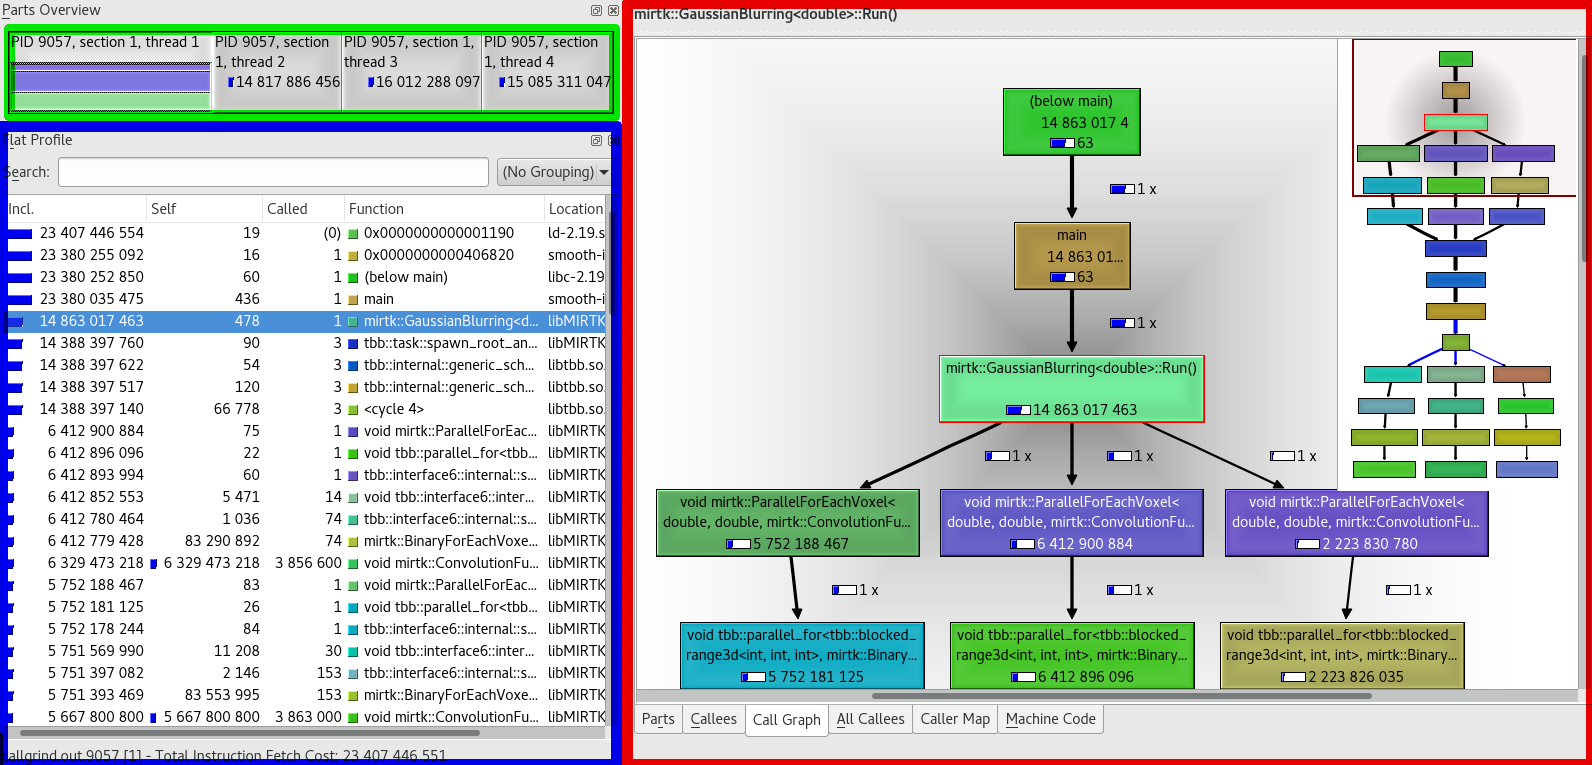
\includegraphics[width=13cm]{Reports/figures/UIkcachegrind.png}
%			\end{center}	
%			\caption{Interface de KCacheGrind pour le profilage}
%			\label{Interface de KCacheGrind pour le profilage}
%		\end{figure}~\par
%		{$\bullet$} \textit{Cadre vert: } Dans cette partie est distinguée tous les threads qui ont exécuté une partie du code lié à l'exécutable étudié. Tous les threads ayant été utilisés dans ce cas, on peut constater que la machine fonctionne donc avec 4 coeurs. \newline
%		{$\bullet$} \textit{Cadre bleu: } Ici est détaillé toutes les fonctions les plus coûteuses du thread sélectionné. \newline
%		{$\bullet$} \textit{Cadre rouge: } Grâce à ce diagramme, on peut visualiser la pile d'appel des fonctions avant et après la fonction sélectionné dans le cadre bleu. Les onglets en bas de page sont d'autres représentations plus textuelles (et plus détaillées) de ce que montre le diagramme. \newline
%		

%		\subsection{Choix du profileur}~\par

%		
%	
%	%	=> on identifie les fonctions sur lesquelles agir en premier
%	%	On utilise Valgrind, qui, avec callgrind analyse la manière dont les caches sont utilisés.
%	%	Expliquer le choix de valgrind, parmi les autres profileurs
%	% => projet open-source multi-plateforme et disponible dans les packages linux, autres alternatives étudiées (VTUNE intel, installation compliquée, et codeXL, valgrindqui nécessite des proc AMD).\\
%		
		\subsubsection{b) Résultats}
		La suite d'outils de Valgrind permet d'étudier deux différents critères au travers de deux modules appelés Callgrind et Cachegrind.\\
		Callgrind va étudier le coût, en nombre d'instructions CPU, des fonctions du programmes profilé. Chaque instruction ayant le même temps d'exécution, le nombre d'instructions est proportionnel au temps. L'évolution relative du nombre d'instructions est donc équivalente à celle du temps d'exécution.\\
		Cachegrind est un module qui simule l'interaction du programme avec la hiérarchie des caches. Les caches représentent une partie de la mémoire informatique, et enregistrent temporairement des copies de données provenant d'une source, afin de diminuer le temps d'un nouvel accès d'un CPU à ces données. Comme représenté en figure \ref{Différents niveaux de mémoire d'un microprocesseur}, il y a plusieurs niveaux de mémoire entre un CPU et sa mémoire principale. 

		\begin{figure}[h!]
			\begin{center}
				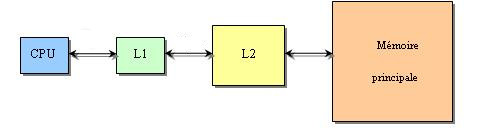
\includegraphics[width=13cm]{Reports/figures/Mem_hierarchy.jpg}
			\end{center}	
			\caption{Différents niveaux de mémoire d'un microprocesseur}
			\label{Différents niveaux de mémoire d'un microprocesseur}
		\end{figure}~\par
		Sur la figure \ref{Différents niveaux de mémoire d'un microprocesseur} sont représenté 2 niveaux de mémoire cache, mais il est possible d'avoir plus ou moins de niveaux.
		Les différents niveaux de mémoire cache sont désignés de la manière suivante : Level 1 (abrégé L1), Level 2 (abrégé L2) ... et le dernier niveau : Last Level (abrégé LL). Les niveaux de cache les plus bas correspondent aux caches les plus proches du CPU. 
		
		\paragraph{Analyse du nombre d'instructions}

		
		\begin{wrapfigure}{r}{7.2cm}
			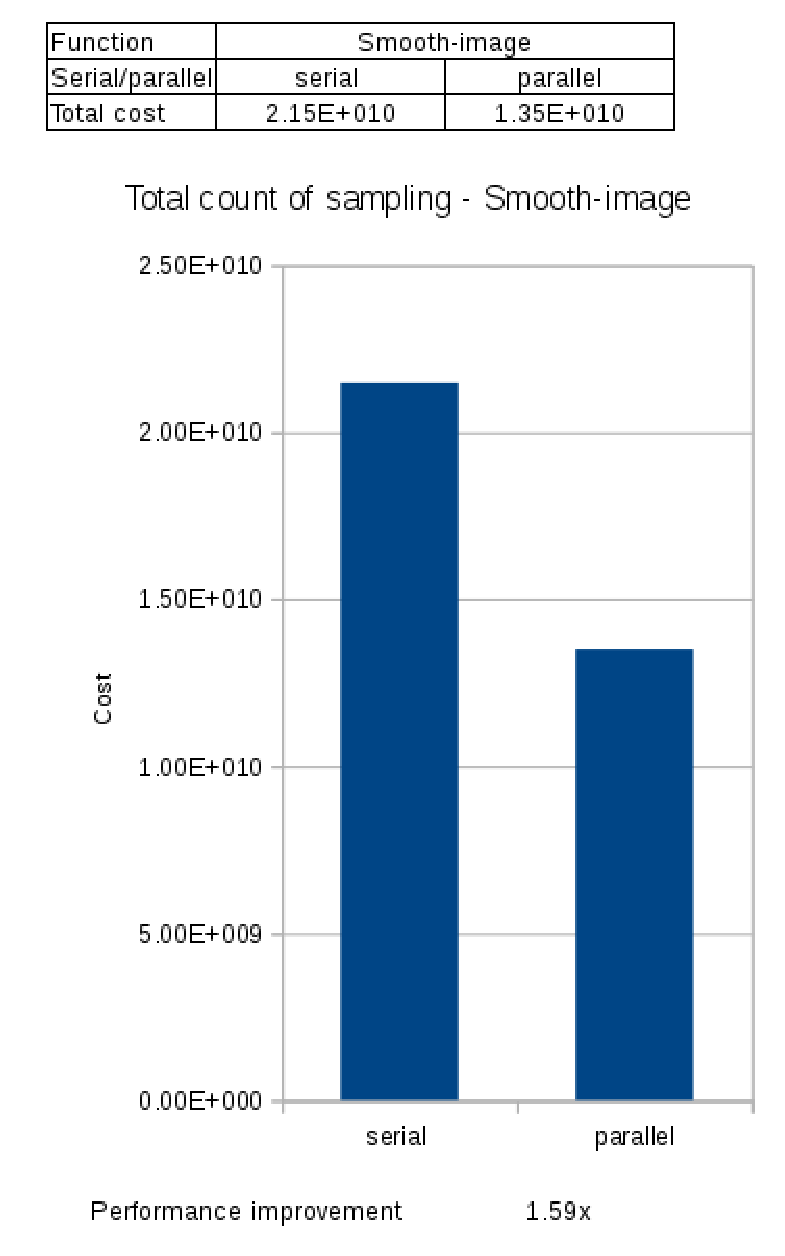
\includegraphics[height=10cm]{Reports/figures/smooth_image_costs.eps}
			\caption{Coût de la fonction de flou gaussien}
			\label{Coût de la fonction de flou gaussien}
		\end{wrapfigure}
%		~\par~\par
%		Dans un premier temps, on s'intéresse au critère le plus pertinent concernant les performances du logiciel. Le nombre d'instructions correspond à la quantité de commandes atomiques (au niveau binaire) exécutées par le CPU et pour chaque thread.
%		Ainsi, on peut étudier l'efficacité de TBB en comparant le nombre d'instructions utilisées lorsque TBB est activé ou non. C'est ce qui est présenté sur l'image présentée ci-contre, en se focalisant sur une fonction de flou gaussien (nommée \textit{smooth-image}).\\
%		Sur l'axe des ordonnées, on a le coût total en instruction de la fonction, appelée sur une machine précise, avec une entrée précise (ici une image 3D). Les résultats dépendent de ces deux critères.Cependant, le ratio entre les coûts de la fonction parallélisée et celle qui ne l'est pas reste sensiblement le même. Au bas de l'image, on peut voir qu'ici, la fonction à un taux d'amélioration de x1.59. L'ordinateur ayant exécuté cette fonction ayant 8 coeurs, on peut dire que ce résultat reflète une mauvaise parallélisation dans ce cas, car un logiciel bien optimisé aurait un taux d'amélioration proche de x8 (équivalent au nombre de coeurs utilisés).\\
%		De même, ci-dessous, l'image décrit les performances de la fonction \textit{transform-image}. En revanche, ici, cette fonction possède une option qui permet de choisir son type d'interpolation mathématique. On a donc fait un test de coût d'instructions pour chaque interpolation et on a relevé ici le taux de performance associé:
		\begin{figure}[h!]
			\begin{center}
				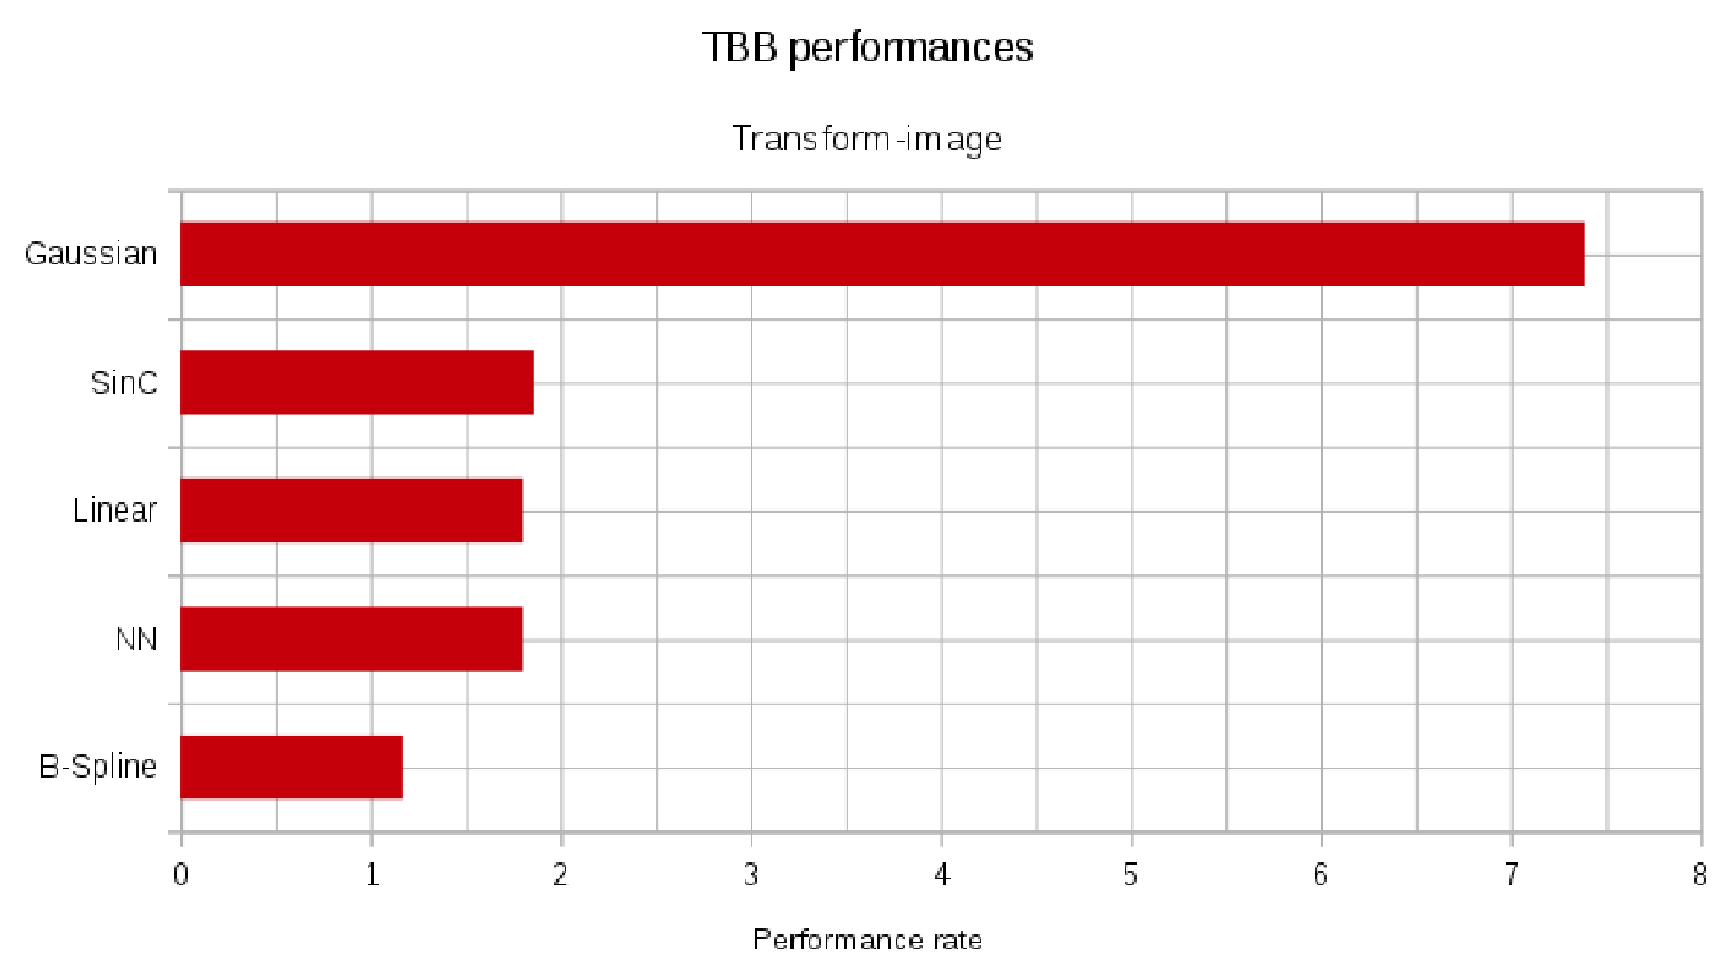
\includegraphics[width=9cm]{Reports/figures/performances_tbb_transform_image.eps}
			\end{center}	
			\caption{Améliorations apportées par TBB pour transform-image}
			\label{Améliorations apportées par TBB pour transform-image}
		\end{figure}~\par
%		L'interpolation gaussienne est donc parfaitement parallélisée, ce qui n'est pas le cas des autres interpolations de \textit{transform-image}.
%		
		\paragraph{Analyse des fuites de cache}~\par
		En plus des fuites de caches, CacheGrind est capable de relever d'autres informations pertinentes telles que les erreur de prédiction de branchement.\\
		La prédiction de branchement est une fonctionnalité d'un processeur qui lui permet de prédire le résultat d'un branchement. Avec cette technique, le processeur va faire de l’exécution spéculative : il va parier sur le résultat d'un branchement, et va poursuivre l’exécution du programme avec le résultat du pari. Si le pari échoue, les instructions chargées par erreur sont annulées. Dans ce cas-ci, CacheGrind relèvera une mauvaise prédiction de branche. \\
		\\Pour "transform-image", CacheGrind indique relativement peu de fuites de caches, mais, en revanche, le taux de mauvaise prédiction de branche vaut entre 10\% et 20\% en fonction de l'interpolation choisie. De plus, le taux de variation des mauvaises prédictions de branches et de fuites de caches est très faibles entre un code sérialisé et un code parallélisé avec les fonctionnalités présentes dans le MIRTK.

			\begin{figure}[h!]
				\begin{center}
					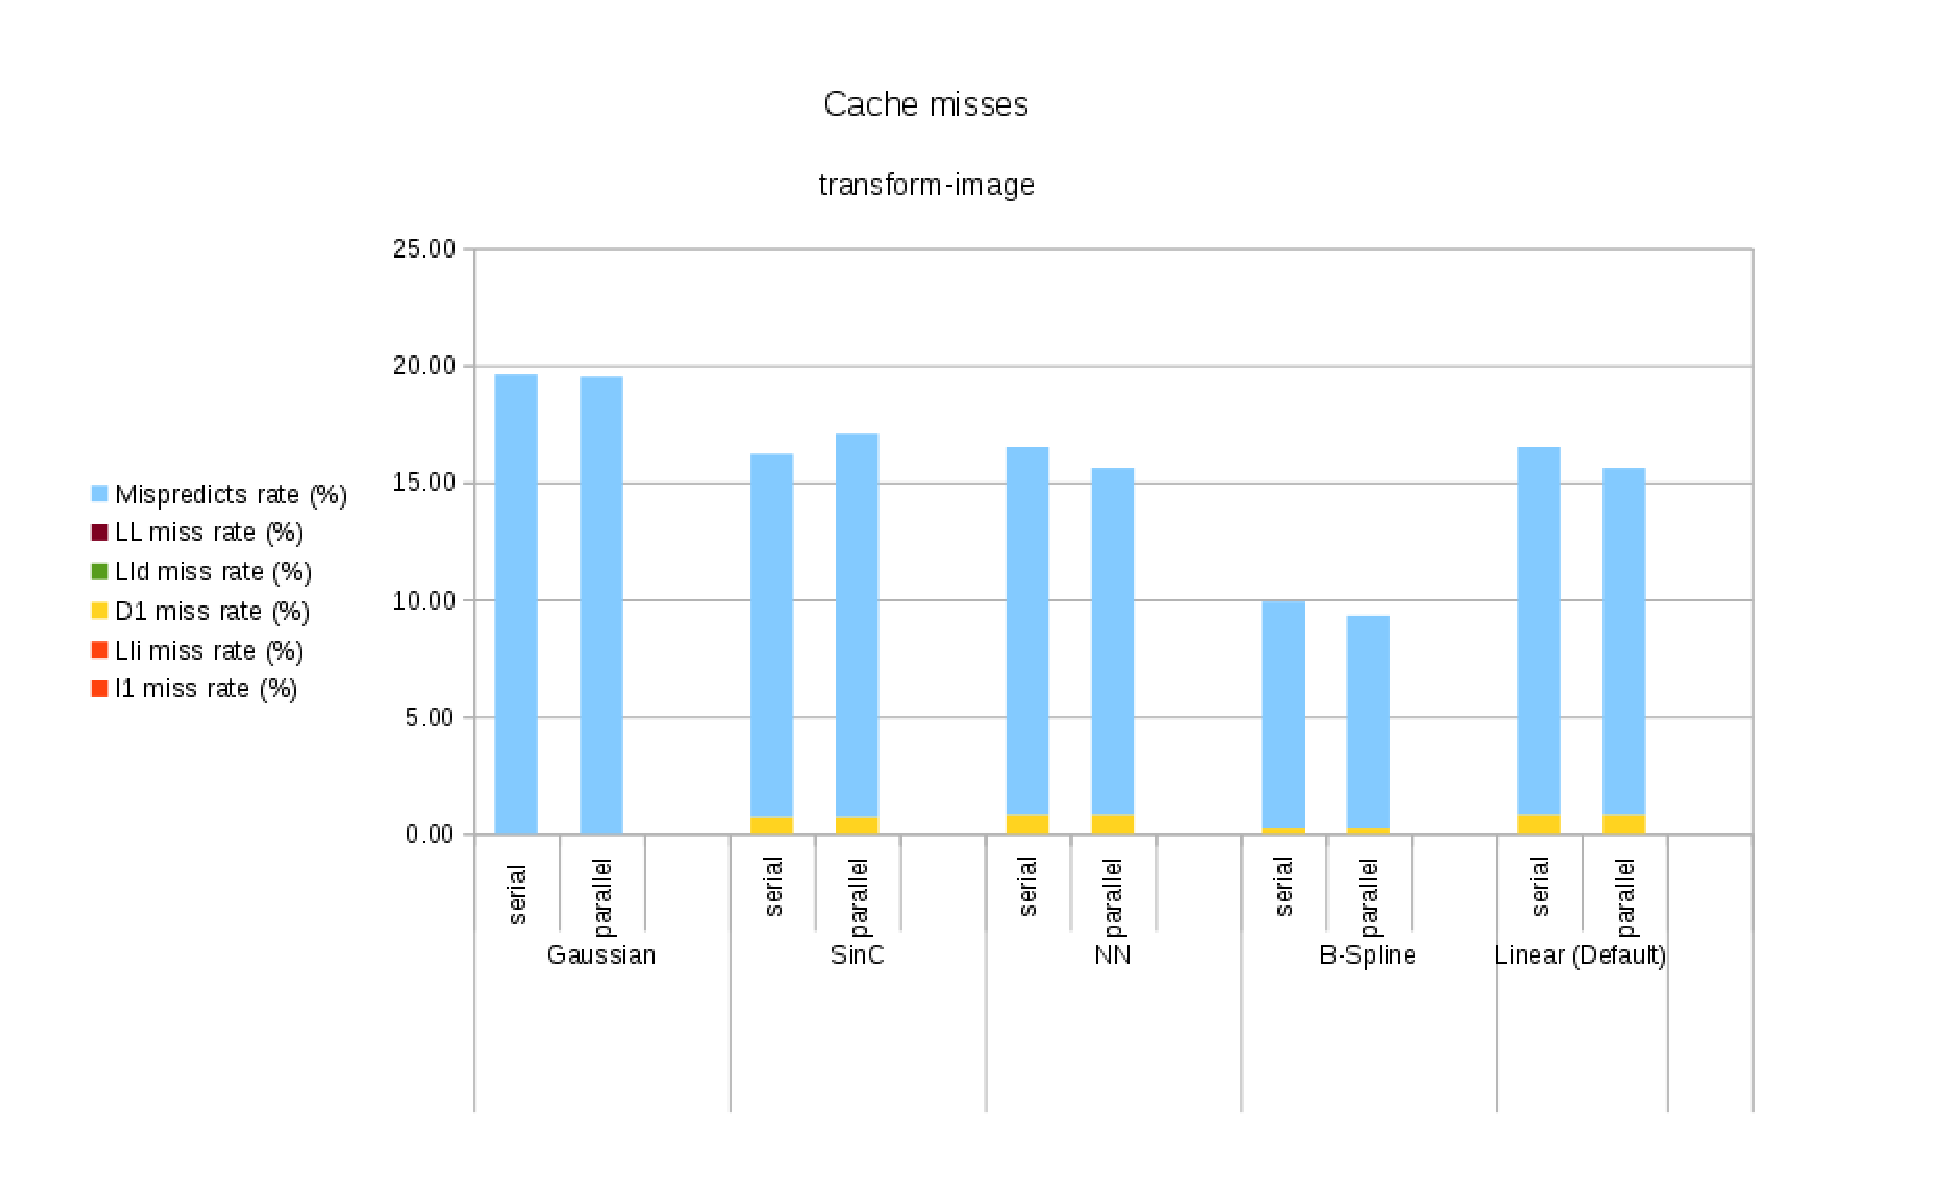
\includegraphics[width=15cm]{Reports/figures/cache_misses_transform_image.eps}
				\end{center}	
				\caption{Fuites de cache pour la fonction transform-image}
				\label{Fuites de cache pour la fonction transform-image}
			\end{figure}~\par

	\subsection{Analyse}
%	(partie dépendante du déroulement du projet)\newline
%	- Analyse des performances obtenues \newline
%	- Comparaison avec le profilage initial ? \newline
%	- Points où il y a eu des concessions (exemple: alourdir le code pour parvenir à un résultat précis)
	
\chapter{Améliorations et perspectives}
	\section{A cours terme}
	Une fois le stage achevé sur le plan technique, les modifications apportées vont parfois annuler l'utilisation de certains attributs et/ou méthodes de classes. Ces variables se retrouveront donc non-utilisées. De même, certaines fonctionnalités d'ArrayFire ont remplacé d'anciennes fonctions du MIRTK, et la présence de doublons est encore possible. L'étape prioritaire après le stage sera de réorganiser la structure du code par réusinage.\\
	\\Par la suite, d'autres fonctions du MIRTK pourront être ré-implémentées avec ArrayFire afin d'encore améliorer les performances du module de recalage du logiciel.

	\section{A long terme}
	Comme détaillé dans les parties 1.2.2 et 2.1, le projet UK BioBank rassemblera d'importantes données d'imagerie. Le logiciel traitant ces images devra être cependant plus performant que le MIRTK actuel. En effet, malgré les résultats prometteurs du stage, la modification des fonctions telle qu'initiée ne permettra pas, à terme d'obtenir un logiciel aux performances optimales. \\
	\\Puisque les concepts logiciels utilisé dans le MIRTK sont, pour l'instant, optimisés pour des calculs sur les voxels de l'image, le MIRTK devra être modifié au niveau de ses structures de données et de ses classes pour favoriser au mieux l'amélioration des performances initiée par ArrayFire. Dans cet optique, il sera nécessaire d'orienter les classes du MIRTK vers des vecteurs et des matrices, et dont les méthodes faciliteront des calculs vectorisés.
%uk biobank
\chapter*{Conclusion} % dans cet ordre
\addcontentsline{toc}{chapter}{Conclusion}
\chapter*{Sources}
\addcontentsline{toc}{chapter}{Sources}
\noindent
\url{https://biomedia.doc.ic.ac.uk/}  : image page de garde, partie du texte 1.1.3 \\
\url{http://www.imperial.ac.uk} : partie du texte 1.1.2 (Department of computing) et schéma stratégie du département\\
\url{https://fr.wikipedia.org/wiki/Imperial_College_London} : partie du texte 1.1.1 (Imperial College London)\\
\url{http://www.ukbiobank.ac.uk/about-biobank-uk/} : inspiration pour le paragraphe 1.2.2 (UK BioBank)\\
\url{http://ric.uthscsa.edu/mango/papaya/index.html} : outil de visualisation d'images en format NIFTI\\
\url{https://wiki.imperial.ac.uk/display/HPC/Systems} : données sur la grille de calcul de l'Imperial College\\
\url{http://www.egi.eu/} : données sur la grille européenne de calcul\\
\url{https://fr.wikipedia.org/wiki/Parall\%C3\%A9lisme_\%28informatique\%29} : définition de la parallélisation, partie 2.1\\
\url{https://fr.wikipedia.org/wiki/R\%C3\%A9usinage_de_code} :  définition d'un réusinage \\
\url{http://www.nvidia.fr/object/gpu-computing-fr.html}: explication du calcul sur GPU en 2.1\\
ProGit\\
\url{https://fr.wikipedia.org/wiki/Pr\%C3\%A9diction_de_branchement}: définition d'une prédiction de branchement.\\
\url{https://fr.wikipedia.org/wiki/Recalage_d'images}: définition du recalage d'images.\\
\renewcommand{\listfigurename}{Table des illustations}\listoffigures 
\addcontentsline{toc}{chapter}{Table des illustrations}
\chapter*{Glossaire}
\addcontentsline{toc}{chapter}{Glossaire}
\noindent
\textbf{Back-end:}\\ 
\textbf{Front-end:}\\
\textbf{Profilage:} Différence avec le benchmarking ?\\
\textbf{Run-time:}\\
\textbf{Fuite de cache:}\\
\textbf{Parangonnage:} Différence avec le profiling ?\\
\textbf{Thread:}\\
\textbf{Prédiction de branche:}\\
\textbf{Fuite de cache:}\\
\textbf{Environnement d'exécution:}\\
\textbf{CPU:}\\
\textbf{GPU:}\\
\textbf{Voxel:}\\
\textbf{Réusinage d'un code (ou \textit{code refactoring}, en anglais):} opération consistant à retravailler le code source d'un programme informatique (sans toutefois y ajouter des fonctionnalités ni en corriger les bogues) de façon à en améliorer la lisibilité et par voie de conséquence la maintenance, ou à le rendre plus générique (afin par exemple de faciliter le passage de simple en multiple précision); on parle aussi de « remaniement ». 
\definecolor{mygreen}{rgb}{0,0.6,0}
\definecolor{mygray}{rgb}{0.5,0.5,0.5}
\definecolor{mymauve}{rgb}{0.58,0,0.82}

\lstset{ %
	backgroundcolor=\color{white},   % choose the background color
	basicstyle=\footnotesize,        % size of fonts used for the code
	breaklines=true,                 % automatic line breaking only at whitespace
	captionpos=b,                    % sets the caption-position to bottom
	commentstyle=\color{mygreen},    % comment style
	escapeinside={\%*}{*)},          % if you want to add LaTeX within your code
	keywordstyle=\color{blue},       % keyword style
	stringstyle=\color{mymauve},     % string literal style
}

\begin{appendix}
	\chapter*{Annexe 1: Implémentation d'une fonction de recherche de valeurs propres en C++}
	\addcontentsline{toc}{chapter}{Annexe 1: Implémentation d'une fonction de recherche de valeurs propres en C++}
\vspace{-1cm}
\begin{lstlisting}[language=C++]
#include <arrayfire.h>
#include <cstdio>
#include <cstdlib>
// A preliminary test has been done to check whether the matrix is square and symmteric or not
af::array EigenValuesSolver(af::array &in) // the input is an array
{
	int size = in.dims(0); // gets dimensions of the input array
	int coltemp = 0;
	int rowtemp = 0;
	unsigned index = 0;
	float maxi = 0;
	float last_value;
	float new_value;
	float threshold = 0.001; // sets a threshhold for the stopping condition of the algorithm
	af::array U = af::identity(size, size);
	af::array V;
	af::array A = in; // copy the input array into a local variable
	af::array alpha = af::constant(1, 1, 1); // stores a numeric variable in an array
	af::array temp;
	
	/* Starts a Jacobi algorithm */
	do
	{
		last_value = maxi; // keeps the previous maximum value of A 
		
		/* Gets the maximum value from A outside its diagonal */
		temp = af::abs(A-af::diag(af::diag(A), 0, false)); 
		af::max(&maxi, &index, temp);  
		rowtemp = index%size;         // gets maximum value's row index
		coltemp = index/size;         // gets maximum value's column index
		
		/* Calculates the new rotation angle */
		alpha = 0.5*atan(2*A(rowtemp, coltemp)/(A(coltemp, coltemp)-A(rowtemp, rowtemp)));
		
		/* Creates the new rotation matrix */
		V = af::identity(size, size);
		V(rowtemp, coltemp) = sin(alpha);
		V(coltemp, coltemp) = cos(alpha);
		V(rowtemp, rowtemp) = cos(alpha);
		V(coltemp, rowtemp) = -sin(alpha);
		
		/* Final multiplications */
		A = af::matmul((af::transpose(V)),A,V); 
		U = af::matmul(U,V);
		
		new_value = maxi; // update the maximum value 
	}while(abs(last_value-new_value) > threshold); // loop condition
	
	return af::diag(A); // eigen values of the input are returned by getting
}

\end{lstlisting}

\chapter*{Annexe 2: Implémentation de "smooth-image" en Python}
\addcontentsline{toc}{chapter}{Annexe 2: Implémentation de "smooth-image" en Python}
\vspace{-1cm}
\begin{lstlisting}[language=python]
import arrayfire as af
import matplotlib.pyplot as plt
import nibabel as nib 
from scipy import signal
import numpy as np
import argparse as ap
	
# Command line arguments and options handling 
parser = ap.ArgumentParser()
parser.add_argument("InputImage", type=str, help="Path to the input image")
parser.add_argument("OutputImage", type=str, help="Path to the input image")
parser.add_argument("Sigma", type=int, help="Defines the value of sigma for the Gaussian kernel. Default: 1")
parser.add_argument("--dimension", type=str, choices=["x", "y", "z", "xy", "yz", "xz", "xyz"], help="Specifies on which dimensions execute the blurring. Default: xyz")
parser.add_argument("-color", help="Enable colored input/output image plot.", action="store_false")
parser.add_argument("-nodisplay", help="Cancel plot of the input/output images. Has priority over \"-color argument\".", action="store_false")

args = parser.parse_args()

# Loading input
img = nib.load(args.InputImage)
hdr = img.get_header()
img_data = img.get_data().astype('f')

# Conversion numpy => arrayfire
img_data_af = af.interop.np_to_af_array(img_data)

# Declaration of Gaussian kernel
if args.Sigma:
	kernel = signal.gaussian(img_data.shape[0], std = args.Sigma).astype('f')
else:
	kernel = signal.gaussian(img_data.shape[0], std = 1).astype('f')

# Conversion numpy => arrayfire for the Gaussian kernel
kernel_af = af.interop.np_to_af_array(kernel)

# Convolution along dimensions chosen 
output_image = img_data_af.copy()
input_image = img_data_af.copy()

if (args.dimension):

	if ("x" in args.dimension):
		output = af.convolve1(input_image, kernel_af)
	
	if ("y" in args.dimension):
		input_image = af.reorder(output_image, 1, 0, 2)
		output_image = af.convolve1(input_image, kernel_af)
		output_image = af.reorder(output_image, 1, 0, 2)
	
	if ("z" in args.dimension):
		input_image = af.reorder(output_image, 2, 1, 0)
		output_image = af.convolve1(input_image, kernel_af)
		output_image = af.reorder(output_image, 2, 1, 0)
else:
	output_image = af.convolve1(input_image, kernel_af)
	input_image = af.reorder(output_image, 1, 0, 2)
	output_image = af.convolve1(input_image, kernel_af)
	output_image = af.reorder(output_image, 1, 0, 2)
	input_image = af.reorder(output_image, 2, 1, 0)
	output_image = af.convolve1(input_image, kernel_af)
	output_image = af.reorder(output_image, 2, 1, 0)


# Conversion arrayfire => numpy
output_np = output_image.to_array()
output_np = np.asarray(output_np)
output_np = output_np.reshape(320, 250, 202, order='F')

# Saving the output file
affine = img.get_affine()
new_img = nib.Nifti1Image(output_np, affine)
nib.save(new_img, args.OutputImage)

# Check if plot is not cancelled by "-nosdisplay" argument
if (args.nodisplay == True):
	# Assimilating color option
	if (args.color):
		colors = 'gray'
	else:
		colors = None
	
	# Ploting 1rst window
	f,fig = plt.subplots(1, 2)
	fig[0].imshow(img_data[125, :, :].T, extent=[0, hdr['pixdim'][1], 0, hdr['pixdim'][3]], cmap=colors, origin='lower')
	fig[1].imshow(output_np[125, :, :].T, extent=[0, hdr['pixdim'][1], 0, hdr['pixdim'][3]], cmap=colors, origin='lower')
	plt.suptitle("Gaussian Blurring on x-axis")
	
	# Ploting 2nd window
	f2,fig2 = plt.subplots(1, 2)
	fig2[0].imshow(img_data[:, 125, :].T, extent=[0, hdr['pixdim'][1], 0, hdr['pixdim'][3]], cmap=colors, origin='lower')
	fig2[1].imshow(output_np[:, 125, :].T, extent=[0, hdr['pixdim'][1], 0, hdr['pixdim'][3]], cmap=colors, origin='lower')
	plt.suptitle("Gaussian Blurring on y-axis")
	
	# Ploting 3rd window
	f3,fig3 = plt.subplots(1, 2)
	fig3[0].imshow(img_data[:, :, 125].T, cmap=colors, origin='lower')
	fig3[1].imshow(output_np[:, :, 125].T, cmap=colors, origin='lower')
	plt.suptitle("Gaussian Blurring on z-axis")
	
	plt.show()
	\end{lstlisting}

\end{appendix}

\end{document}
